% THIS DOCUMENT IS FOLLOWS THE VOLERE TEMPLATE BY Suzanne Robertson and James Robertson
% ONLY THE SECTION HEADINGS ARE PROVIDED
%
% Initial draft from https://github.com/Dieblich/volere
%
% Risks are removed because they are covered by the Hazard Analysis
\documentclass[11pt]{article}

\usepackage{booktabs}
\usepackage{tabularx}
\usepackage{hyperref}
\usepackage{float}
\usepackage{graphicx} 
\usepackage{longtable}
\usepackage{geometry}
\usepackage{ltablex}

\keepXColumns

\hypersetup{
    bookmarks=true,         % show bookmarks bar?
      colorlinks=true,      % false: boxed links; true: colored links
    linkcolor=red,          % color of internal links (change box color with linkbordercolor)
    citecolor=green,        % color of links to bibliography
    filecolor=magenta,      % color of file links
    urlcolor=cyan           % color of external links
}

\geometry{a4paper, margin=1in}

\newcommand{\lips}{\textit{Insert your content here.}}

%% Comments

\usepackage{color}

\newif\ifcomments\commentstrue %displays comments
%\newif\ifcomments\commentsfalse %so that comments do not display

\ifcomments
\newcommand{\authornote}[3]{\textcolor{#1}{[#3 ---#2]}}
\newcommand{\todo}[1]{\textcolor{red}{[TODO: #1]}}
\else
\newcommand{\authornote}[3]{}
\newcommand{\todo}[1]{}
\fi

\newcommand{\wss}[1]{\authornote{magenta}{SS}{#1}} 
\newcommand{\plt}[1]{\authornote{cyan}{TPLT}{#1}} %For explanation of the template
\newcommand{\an}[1]{\authornote{cyan}{Author}{#1}}

%% Common Parts

\newcommand{\progname}{Software Engineering} % PUT YOUR PROGRAM NAME HERE
\newcommand{\authname}{Team 13, Speech Buddies
\\ Mazen Youssef
\\ Rawan Mahdi
\\ Luna Aljammal
\\ Kelvin Yu} % AUTHOR NAMES                  

\usepackage{hyperref}
    \hypersetup{colorlinks=true, linkcolor=blue, citecolor=blue, filecolor=blue,
                urlcolor=blue, unicode=false}
    \urlstyle{same}
                                


\begin{document}

\title{Software Requirements Specification for \progname: subtitle describing software} 
\author{\authname}
\date{\today}
	
\maketitle

~\newpage

\pagenumbering{arabic}

\tableofcontents

~\newpage

\section*{Revision History}

\begin{tabularx}{\textwidth}{p{3cm}p{2cm}X}
\toprule {\textbf{Date}} & {\textbf{Version}} & {\textbf{Notes}}\\
\midrule
October 2, 2025 & Rawan and Luna & Filled-In Initial Draft of SRS Document\\
October 10, 2025 & Rawan and Luna & Completed SRS Document\\

\bottomrule
\end{tabularx}

~\\

~\newpage
\section{Purpose of the Project}
\subsection{User Business}


Individuals with speech impairments face significant barriers when interacting with digital devices. VoiceBridge addresses this gap by providing an accurate, inclusive, and accessible speech-to-control system that enables users to communicate with their devices using their speech, regardless of clarity of articulation. Building on familiar technology, such as personal computers and mobile devices, may be one of the most cost-effective and easily adoptable approaches for improving an individual with disability’s autonomy and access to the world around them. The rise of ASR technology and Artificial Intelligence (AI) integrations in the industry provides a novel landscape of opportunities to improve accessibility interfaces. VoiceBridge exploits bleeding-edge technology for a practical and impactful application.

\subsection{Goals of the Project}
\begin{table}[H]
\centering
\begin{tabularx}{\textwidth}{p{1cm}p{4cm}p{8cm}X}
\toprule {\textbf{ID}} & {\textbf{Goal}} & {\textbf{Description}}\\
\midrule
G1 & \textbf{Accurate Speech Transcription} & Reliably convert impaired or slurred speech into text. \\ \hline
G2 & \textbf{Command Mapping} & Translate recognized speech into actionable browser commands. \\ \hline
G3 & \textbf{User Independence} & Enable users with speech impairments to browse autonomously. \\ \hline
G4 & \textbf{Lightweight \& Accessible Design} & Keep the system simple, fast, and cost-effective. \\ \hline
G5 & \textbf{Cross-Browser Compatibility} & Support major browsers (e.g., Chrome, Edge, Firefox). \\ \hline
G6 & \textbf{Robust Error Handling} & Detect and recover gracefully from common failures. \\ \hline
G7 & \textbf{Data Privacy \& Security} & Protect user data and ensure secure local processing. \\ \hline
G8 & \textbf{Customizable Interface} & Allow users to adjust sensitivity, shortcuts, and feedback modes. \\ \hline
G9 & \textbf{Scalable Architecture} & Design the system for future integration beyond browsers. \\ \hline
\bottomrule
\end{tabularx}
\caption{Project Goals for VoiceBridge}
\label{tab:project-goals}
\end{table}


\section{Stakeholders}
\subsection{Client}
The primary client for the VoiceBridge project is the organization or individual funding or commissioning the system. The client is primarily concerned with achieving the following goals: \textbf{\hyperref[tab:project-goals]{G1}}, \textbf{\hyperref[tab:project-goals]{G5}}, and \textbf{\hyperref[tab:project-goals]{G9}}, ensuring accurate speech transcription, cross-browser compatibility, and scalable architecture.

\subsection{Customer \& Hands-On Users of the Project}

The primary customers are also the users of the project, them being individuals with speech impairments, who seek independence and autonomy through technology. Their needs directly relate to: \textbf{\hyperref[tab:project-goals]{G1}}, \textbf{\hyperref[tab:project-goals]{G2}}, \textbf{\hyperref[tab:project-goals]{G3}}, and \textbf{\hyperref[tab:project-goals]{G8}}.

\subsection{Other Stakeholders}
Secondary stakeholders include experts in linguistics, speech processing, and healthcare domains:
\begin{itemize}
    \item Speech researchers and linguistics specialists, including the project supervisor, Dr. Christian Brodbeck, who provide insight toward \textbf{\hyperref[tab:project-goals]{G1}} and \textbf{\hyperref[tab:project-goals]{G6}}.
    \item Healthcare professionals and speech therapists who advise on usability and accessibility, contributing to \textbf{\hyperref[tab:project-goals]{G3}} and \textbf{\hyperref[tab:project-goals]{G8}}.
    \item Accessibility advocates and organizations interested in promoting the application, aligned with \textbf{\hyperref[tab:project-goals]{G4}} and \textbf{\hyperref[tab:project-goals]{G5}}.
    \item Software developers who implement and maintain the system, supporting \textbf{\hyperref[tab:project-goals]{G9}} and \textbf{\hyperref[tab:project-goals]{G6}}.
\end{itemize}

Tertiary stakeholders include caregivers and professionals who interact with end users, supporting \textbf{\hyperref[tab:project-goals]{G3}} and \textbf{\hyperref[tab:project-goals]{G7}}.

\subsection{Personas}

Potential end users of VoiceBridge include:
\begin{itemize}
    \item \textbf{Amira}, a 45-year-old with Parkinson’s disease, uses the system to log into Gmail and send emails.
    \item \textbf{David}, a stroke survivor, uses the system to browse the web and make purchases.
\end{itemize}


\subsection{Priorities Assigned to Users}

The highest priorities are assigned to end users with speech impairments, as their experience with the system defines its success. Secondary priorities include caregivers and technical experts who support the end users in using and maintaining the system.

\subsection{User Participation}

Individuals matching the target user profiles will be recruited for prototype testing and personalization development. Their participation directly supports refining goals \textbf{\hyperref[tab:project-goals]{G1}}, \textbf{\hyperref[tab:project-goals]{G2}}, \textbf{\hyperref[tab:project-goals]{G3}}, and \textbf{\hyperref[tab:project-goals]{G8}}.

\subsection{Maintenance Users and Service Technicians}
\textbf{Maintenance Users:}\\
\hrule
\begin{itemize}
    \item \textbf{Role:} End-users or caregivers performing basic troubleshooting and initiating support requests.
    \item \textbf{Responsibilities:} 
        \begin{itemize}
            \item Reporting errors or unexpected system behavior (\textbf{\hyperref[tab:project-goals]{G6}}).
            \item Installing application updates (\textbf{\hyperref[tab:project-goals]{G9}}).
            \item Managing user-specific configurations (\textbf{\hyperref[tab:project-goals]{G8}}).
        \end{itemize}
\end{itemize}
\vspace{1em}
\textbf{Service Technicians:}\\
\hrule
\begin{itemize}
    \item \textbf{Role:} Trained technical staff with deeper access to system logs and back-end services.
    \item \textbf{Responsibilities:}
        \begin{itemize}
            \item Investigating reported issues (\textbf{\hyperref[tab:project-goals]{G6}}).
            \item Ensuring transcription accuracy (\textbf{\hyperref[tab:project-goals]{G1}}).
            \item Deploying updates and patches (\textbf{\hyperref[tab:project-goals]{G9}}).
            \item Ensuring compatibility with operating systems and accessibility frameworks (\textbf{\hyperref[tab:project-goals]{G5}}).
            \item Performing preventive maintenance, including performance monitoring and optimization (\textbf{\hyperref[tab:project-goals]{G1}}, \textbf{\hyperref[tab:project-goals]{G6}}).
        \end{itemize}
\end{itemize}


\section{Mandated Constraints}
\subsection{Solution Constraints}

\begin{tabularx}{\textwidth}{p{1cm}X X X}
\toprule
\textbf{ID} & \textbf{Constraint} & \textbf{Rationale} & \textbf{Fit Criterion} \\
\midrule
C1 & The product shall run on consumer-grade hardware using a personal computer microphone and support macOS, Windows, and Linux distributions. & Requiring only consumer-grade hardware ensures broad accessibility for end users and avoids dependency on specialized equipment. & The system must successfully be integrated onto browsers and run on laptops or desktops across the supported operating systems, using either built-in or external microphones. \\
\hline
C2 & The product shall accept non-deterministic user input in the form of natural language speech. & Individuals with speech impairments may produce varied speech patterns that cannot be handled by rigid or deterministic command structures. & The system must be capable of processing and responding to variable natural language inputs without requiring a fixed set of commands. \\
\hline
C3 & The product shall integrate with a browser control application to execute voice-based commands. & Browser interaction is a primary accessibility point for most digital services, and browser control is essential for practical use of the system. & The system must successfully perform browser actions (e.g., opening tabs, navigating to URLs, scrolling) through the integrated control application. \\
\bottomrule
\end{tabularx}


\subsection{Implementation Environment of the Current System}


\begin{tabularx}{\textwidth}{p{1cm}X X X}
\toprule
\textbf{ID} & \textbf{Constraint} & \textbf{Rationale} & \textbf{Fit Criterion} \\
\midrule
C4 & The product will operate within a consumer computing environment consisting of personal computers equipped with microphones. & This setup reflects the most common user hardware configuration, ensuring the solution is accessible without additional devices. & All core functionalities must operate correctly on standard personal computers with a functioning audio input device. \\
\bottomrule
\end{tabularx}

\subsection{Partner or Collaborative Applications}


\begin{tabularx}{\textwidth}{p{1cm}X X X}
\toprule
\textbf{ID} & \textbf{Constraint} & \textbf{Rationale} & \textbf{Fit Criterion} \\
\midrule
C5 & The initial integration target is Browser Use, an open-source browser control and automation application. & Leveraging existing open-source browser automation tools accelerates development and reduces implementation complexity. & The system must demonstrate the ability to execute at least three browser actions through the integrated partner application during testing. \\
\hline
C6 & Future integrations may include API servers, mobile device agents, and home assistants to extend accessibility and functionality. & Ensuring extensibility allows the system to grow and adapt to new platforms or user needs. & The system architecture must allow seamless integration with additional partner applications without major redesign. \\
\bottomrule
\end{tabularx}

\subsection{Off-the-Shelf Software}

\begin{tabularx}{\textwidth}{p{1cm}X X X}
\toprule
\textbf{ID} & \textbf{Constraint} & \textbf{Rationale} & \textbf{Fit Criterion} \\
\midrule
C7 & The product will rely on off-the-shelf software components, specifically Browser Use for automation and Project Euphonia for voice recording. & Using established open-source components allows focus on core functionality, improves maintainability, and supports experimentation with real-world data. & These components must be successfully integrated into the development workflow, and collected recordings must be stored and processed for model training without licensing conflicts. \\
\bottomrule
\end{tabularx}

\subsection{Anticipated Workplace Environment}


\begin{tabularx}{\textwidth}{p{1cm}X X X}
\toprule
\textbf{ID} & \textbf{Constraint} & \textbf{Rationale} & \textbf{Fit Criterion} \\
\midrule
C8 & The product may be used at home, in public spaces, or in clinical settings, each with varying background noise conditions. & The product must function effectively across diverse real-world environments to meet accessibility goals. & The speech recognition system must maintain acceptable accuracy and responsiveness across all three identified environments during testing. \\
\bottomrule
\end{tabularx}


\subsection{Schedule Constraints}


\begin{tabularx}{\textwidth}{p{1cm}X X X}

\toprule
\textbf{ID} & \textbf{Constraint} & \textbf{Rationale} & \textbf{Fit Criterion} \\
\midrule
C9 & Proof of concept must be completed by November 17, 2025. MVP must be ready within eight months, by May 2026. & Deadlines align with capstone project milestones and funding timelines, ensuring timely testing and delivery. & All proof of concept requirements must be met by the November deadline, and MVP functionality must be fully operational by May 2026. \\
\bottomrule
\end{tabularx}

\subsection{Budget Constraints}

\begin{tabularx}{\textwidth}{p{1cm}X X X}
\toprule
\textbf{ID} & \textbf{Constraint} & \textbf{Rationale} & \textbf{Fit Criterion} \\
\midrule
C10 & The project must operate within the capstone budget allocated for compute infrastructure and development resources. & Budget limitations require prioritizing open-source solutions and efficient resource allocation. & Total cost of infrastructure, hosting, and third-party services must not exceed the allocated capstone budget. \\
\bottomrule
\end{tabularx}


\subsection{Enterprise Constraints}

\begin{tabularx}{\textwidth}{p{1cm}X X X}
\toprule
\textbf{ID} & \textbf{Constraint} & \textbf{Rationale} & \textbf{Fit Criterion} \\
\midrule
C11 & The product must comply with all relevant accessibility and privacy regulations, including data usage and user privacy agreements. & Compliance protects user rights, upholds institutional standards, and avoids legal or ethical issues. & All data collection and processing workflows must undergo compliance review, and accessibility features must align with recognized standards (e.g., WCAG). \\
\bottomrule
\end{tabularx}

\section{Naming Conventions and Terminology}
\subsection{Glossary of All Terms, Including Acronyms, Used by Stakeholders
involved in the Project}

\lips

\subsection{Technical Terminology}
\textbf{ASR} - Automatic Speech Recognition \\
\textbf{TTS} - Text To Speech \\
\textbf{STT} - Speech To Text \\


\subsection{Medical Terminology}
\textbf{Aphasia} - A condition that robs you of the ability to communicate. It can affect your ability to speak, write and understand language, both verbal and written. Aphasia usually occurs suddenly after a stroke or a head injury. But it can also come on gradually, as in the case of a brain tumor or a progressive neurological disease. \\
\textbf{ALS} - Amyotrophic Lateral Sclerosis \\
\textbf{Dysarthria} - A motor speech disorder that makes it hard to speak. It is caused by damage to the nervous system, which can affect the muscles used for speaking. People with dysarthria may have slurred or slow speech, and they may have difficulty controlling the pitch, volume, and rhythm of their speech. \\

\section{Relevant Facts And Assumptions}
\subsection{Relevant Facts}

\begin{table}[H]
\centering
\begin{tabularx}{\textwidth}{p{1cm}p{6cm}X}
\toprule {\textbf{Fact ID}} & {\textbf{Fact}} & {\textbf{Explanation / Relevance}}\\
\midrule
F1 & \textbf{Users experience speech impairments of varying severity.} & VoiceBridge must handle varying speech clarity, from slurred to partially formed words (related to (\textbf{\hyperref[tab:project-goals]{G1}}), (\textbf{\hyperref[tab:project-goals]{G2}})). \\ \hline
F2 & \textbf{Users want to communicate and navigate independently.} & Motivates autonomy in using the system without reliance on caretakers (supports (\textbf{\hyperref[tab:project-goals]{G3}})). \\ \hline
F3 & \textbf{Users may have limited mobility.} & Hands-free operation improves accessibility and inclusion (supports (\textbf{\hyperref[tab:project-goals]{G3}}), (\textbf{\hyperref[tab:project-goals]{G4}})). \\ \hline
F4 & \textbf{Users value simplicity and low cognitive load.} & Commands should remain intuitive and easy to use (supports (\textbf{\hyperref[tab:project-goals]{G4}})). \\ \hline
F5 & \textbf{Users may have emotional sensitivity around speech difficulty.} & Interface should be respectful and encouraging without repeating goals (complements (\textbf{\hyperref[tab:project-goals]{G6}})). \\ \hline
F6 & \textbf{Users expect privacy and dignity.} & Data handling should preserve privacy and transparency (supports (\textbf{\hyperref[tab:project-goals]{G7}})). \\ \hline
F7 & \textbf{Users may use different languages or accents.} & System must accommodate linguistic diversity without bias (relates to (\textbf{\hyperref[tab:project-goals]{G1}}), (\textbf{\hyperref[tab:project-goals]{G8}})). \\ \hline
F8 & \textbf{Users may use assistive tools concurrently.} & VoiceBridge should integrate seamlessly with other accessibility tools (supports (\textbf{\hyperref[tab:project-goals]{G4}}), (\textbf{\hyperref[tab:project-goals]{G8}})). \\ \hline
F9 & \textbf{Users will vary in technical comfort.} & Onboarding should be minimal and low-friction (supports (\textbf{\hyperref[tab:project-goals]{G4}}), (\textbf{\hyperref[tab:project-goals]{G8}})). \\ \hline
F10 & \textbf{Users appreciate visual feedback and control.} & Feedback builds trust and reduces frustration (complements (\textbf{\hyperref[tab:project-goals]{G1}}), (\textbf{\hyperref[tab:project-goals]{G8}})). \\
\bottomrule
\end{tabularx}
\caption{User-Centered Facts for VoiceBridge with references to project goals}
\label{tab:user-facts}
\end{table}



\subsection{Business Rules}

\begin{table}[H]
\centering
\begin{tabularx}{\textwidth}{p{1cm} X X}
\toprule
\textbf{ID} & \textbf{Business Rule} & \textbf{Rationale} \\
\midrule
BR1 & Users must be able to cancel or stop a command at any time. & Empowers users and prevents frustration. (\hyperref[tab:project-goals]{G3}, \hyperref[tab:project-goals]{G4}) \\
BR2 & Transcribed text must be displayed for user verification before executing critical commands. & Ensures accuracy, avoids misinterpretation, and maintains user confidence, inline with (\hyperref[tab:project-goals]{G1}) \\
BR3 & Browser commands must not execute without user consent for actions with potential data impact (e.g., sending messages, closing tabs). & Protects user privacy and prevents accidental operations. (\hyperref[tab:project-goals]{G2}, \hyperref[tab:project-goals]{G7}) \\
BR4 & The system should provide immediate visual feedback within 5 seconds of speech input. & Builds trust, transparency, and usability for impaired users. (\hyperref[tab:project-goals]{G6}, \hyperref[tab:project-goals]{G1}) \\
BR5 & System must handle moderate background noise without significant degradation of performance. & Maintains reliability in real-world environments.(\hyperref[tab:project-goals]{G1}, \hyperref[tab:project-goals]{G6}) \\
BR6 & Users should be able to configure simple command mappings for personalized tasks. & Supports individual preferences and improves user autonomy. (\hyperref[tab:project-goals]{G2}, \hyperref[tab:project-goals]{G3}, \hyperref[tab:project-goals]{G8}) \\
\bottomrule
\end{tabularx}
\caption{Business Rules for VoiceBridge}
\label{tab:business-rules}
\end{table}


\subsection{Assumptions}
\begin{table}[H]
\centering
\begin{tabularx}{\textwidth}{p{1cm}p{6cm}X}
\toprule {\textbf{ID}} & {\textbf{Assumption}} & {\textbf{Implication for Design}}\\
\midrule
A1 & \textbf{Users have access to a working microphone and modern browser.} & The system assumes functional input hardware and browser APIs for speech capture (see \hyperref[tab:project-goals]{G1}, \hyperref[tab:project-goals]{G5}). \\ \hline
A2 & \textbf{Users will tolerate minor transcription errors if quickly correctable.} & Fast feedback and correction options are more important than perfect accuracy (see \hyperref[tab:project-goals]{G1}, \hyperref[tab:project-goals]{G6}). \\ \hline
A3 & \textbf{Users are willing to train or calibrate the model briefly.} & A short setup phase (e.g., sample phrases) can improve recognition quality (see \hyperref[tab:project-goals]{G1}, \hyperref[tab:project-goals]{G8}). \\ \hline
A4 & \textbf{Users prefer transparent, explainable behavior.} & VoiceBridge should indicate what command is being executed to prevent confusion or mistrust (see \hyperref[tab:project-goals]{G8}). \\ \hline
A5 & \textbf{Users may be in noisy or uncontrolled environments.} & Noise-robust models and confirmation prompts are required to maintain reliability (see \hyperref[tab:project-goals]{G1}, \hyperref[tab:project-goals]{G6}). \\ \hline
A6 & \textbf{Users want emotional ease of use.} & Tone and interface language must feel supportive — e.g., “Let’s try again” instead of “Error” (see \hyperref[tab:project-goals]{G6}). \\ \hline
A7 & \textbf{Users will likely use the tool for daily web tasks.} & The feature set should prioritize essential browser actions (navigation, scrolling, typing, tab control) (see \hyperref[tab:project-goals]{G2}, \hyperref[tab:project-goals]{G3}, \hyperref[tab:project-goals]{G8}). \\
\bottomrule
\end{tabularx}
\caption{Design Assumptions for VoiceBridge with references to related project goals (\textbf{Goals Table \ref{tab:project-goals}}).}
\label{tab:assumptions}
\end{table}

\section{The Scope of the Work}
\subsection{The Current Situation}

Individuals with speech impairments currently rely on standard speech-to-text or manual input to use browsers and devices. Existing systems struggle with slurred or atypical speech, often requiring caregiver assistance.

Typical workarounds include typing commands, using alternative inputs, or correcting errors, leading to frustration and limited autonomy.

Current workflow:
User speaks → Standard recognition → Frequent errors → Manual/caregiver correction → Action executed

VoiceBridge aims to replace this with accurate transcription, command mapping, and immediate feedback, enabling independent browser control.

\subsection{The Context of the Work}

\begin{figure}[H]
\centering
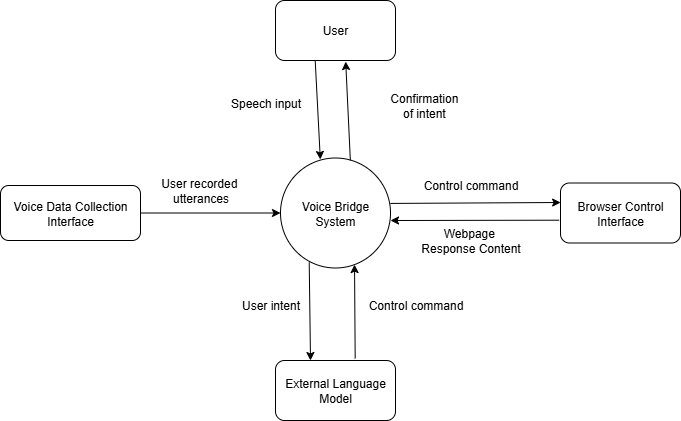
\includegraphics[width=1\textwidth]{../imgs/VoiceBridge_context_diagram.png}
\caption{Context Diagram of VoiceBridge}
\label{fig:voicebridge-context}
\end{figure}

\subsection{Work Partitioning}
\begin{table}[H]
\centering
\begin{tabularx}{\textwidth}{X X X X X}
\toprule
\textbf{Event Name} & \textbf{Input} & \textbf{Output} & \textbf{Brief BUC Summary} & \textbf{Relevant Data Classes} \\
\midrule
\textbf{Input Capture} & User speech via microphone & Audio stream to system & Capture speech for processing & Raw audio, timestamp \\
\hline
\textbf{Speech-to-Text Modelling} & Audio stream & Transcribed text & Convert impaired speech to text & Audio data, transcription \\
\hline
\textbf{Intent Confirmation} & Transcribed text & User confirmation & Verify intended command & Text data, confidence score \\
\hline
\textbf{Command Mapping} & Confirmed text & Actionable command & Map text to browser action & Command definitions, user preferences \\
\hline
\textbf{Browser Interaction Layer} & Actionable command & Executed browser action & Perform command in browser & Command data, page context, execution status \\
\bottomrule
\end{tabularx}
\caption{VoiceBridge Events, Inputs, Outputs, and Data Classes}
\label{tab:voicebridge-events}
\end{table}

% \subsection{Specifying a Business Use Case (BUC)} insert diagram
% \lips

\section{Business Data Model and Data Dictionary}
\subsection{Business Data Model}
\begin{figure}[H]
    \centering
    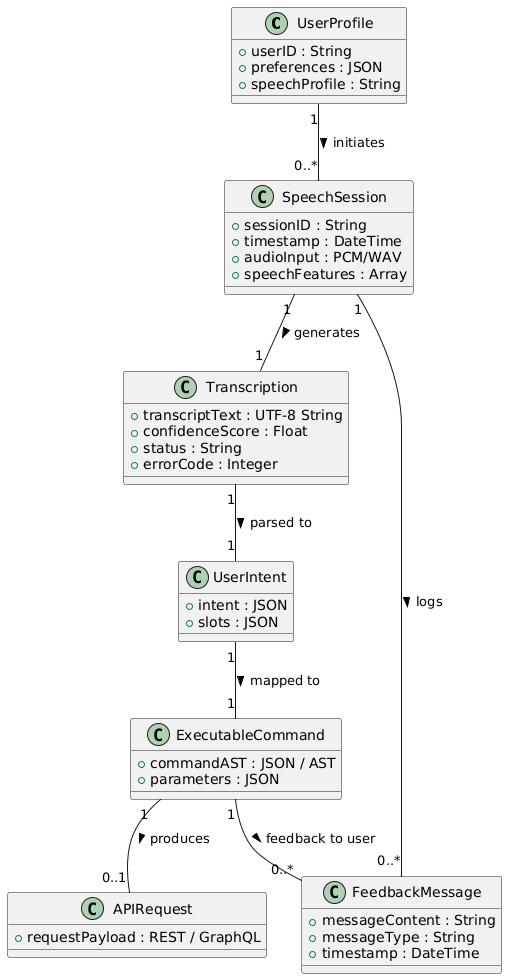
\includegraphics[width=0.7\textwidth]{..//imgs/VoiceBridge_uml.png}
    \caption{VoiceBridge UML Diagram. }
    \label{fig:voicebridge-usecase}
\end{figure} 

\subsection{Data Dictionary}

% \begin{table}[H]
% \centering
% \begin{tabularx}{\textwidth}{p{3cm} X X X X X}
% \toprule
% \textbf{Data Element} & \textbf{Description} & \textbf{Format / Constraints} & \textbf{Source} & \textbf{Remarks / Usage} \\
% \midrule
% Audio\_Input & Raw speech signal captured from microphone &  PCM, WAV, 16 kHz, 16-bit & User microphone & Primary input for ASR processing \\
% Speech\_Features & Extracted features (e.g., MFCCs, spectrogram)  & N-dimensional array & Feature extractor module & Internal representation for ASR engine \\
% Transcript\_Text & Recognized text from speech input & UTF-8 encoded, free text & ASR engine & Used to interpret user intent \\
% Error\_Code & Status / error indicator & Integer &  ASR engine / Controller & 0 = Success, >0 = specific error \\
% User\_Profile & Speaker-specific data (e.g., ID, preferences)  & JSON object & User database & Improves personalization (optional) \\
% Timestamp & Time marker of recognition event & DateTime  & System clock & For logging and debugging \\
% User\_Intent & Parsed intent from natural language & JSON with intent and slots & Interpreter module & Represents structured meaning (e.g., \{“intent”: “open\_file”, “file”: “report.pdf”\}) \\
% Executable\_Command & Structured representation of command before execution & JSON object or Abstract Syntax Tree & Interpreter module & Maps NL to executable form, independent of target system \\
% API\_Request & Finalized API call (if system integration is via APIs)  & REST / GraphQL format & Interpreter module → API translator & Sent to target system \\
% \bottomrule
% \end{tabularx}
% \caption{VoiceBridge Data Elements and Their Usage}
% \label{tab:voicebridge-data-elements}
% \end{table}
% \begin{table}[H]
% \centering
% \caption{VoiceBridge Business Data Model}
% \begin{tabularx}{\textwidth}{p{3cm}X p{2.8cm} p{2.8cm} X}
% \toprule
% \textbf{Entity / Field} & \textbf{Description} & \textbf{Data Type / Format} & \textbf{Source / Owner} & \textbf{Purpose / Usage} \\
% \midrule

% \textbf{Audio\_Input} & Raw speech signal captured from microphone & PCM, WAV, 16 kHz, 16-bit & User microphone & Primary input for ASR processing \\

% \textbf{Speech\_Features} & Extracted acoustic features (e.g., MFCCs, spectrogram) & N-dimensional array & Feature extractor module & Internal representation used by ASR engine \\

% \textbf{Transcript\_Text} & Recognized text output from speech input & UTF-8 encoded free text & ASR engine & Basis for interpreting user intent \\

% \textbf{Error\_Code} & Status or error indicator for system response & Integer & ASR engine / Controller & 0 = Success, >0 = specific error type \\

% \textbf{User\_Profile} & Speaker-specific data such as ID, preferences, and speech patterns & JSON object & User database & Enables personalized recognition and response \\

% \textbf{Timestamp} & Time marker for recognition or command event & DateTime & System clock & Used for logging, debugging, and tracking \\

% \textbf{User\_Intent} & Parsed intent derived from natural language input & JSON (intent and slots) & Interpreter module & Structured meaning representation (e.g., \{“intent”: “open\_file”, “file”: “report.pdf”\}) \\

% \textbf{Executable\_Command} & Structured command before browser execution & JSON object or Abstract Syntax Tree & Interpreter module & Translates user intent into executable browser actions \\

% \textbf{API\_Request} & Outgoing request to external or browser API & REST / GraphQL formatted message & Interpreter module → API translator & Executes command or triggers action in external system \\

% \textbf{Feedback\_Message} & User-facing feedback or error output & String / Audio / JSON & VoiceBridge UI & Confirms action success or requests clarification \\

% \textbf{Session\_ID} & Unique identifier for a single user interaction session & UUID / String & System controller & Links data objects across a single speech-to-command event \\

% \bottomrule
% \end{tabularx}
% \label{tab:business-data-model}
% \end{table}


\begin{tabularx}{\textwidth}{p{3cm} X p{2.8cm} p{2.8cm} X}
\toprule
\textbf{Entity / Field} & \textbf{Description} & \textbf{Data Type / Format} & \textbf{Source / Owner} & \textbf{Purpose / Usage} \\
\midrule

\textbf{Audio\_Input} & Raw speech signal captured from microphone & PCM, WAV, 16 kHz, 16-bit & User microphone & Primary input for ASR processing \\

\textbf{Speech\_Features} & Extracted acoustic features (e.g., MFCCs, spectrogram) & N-dimensional array & Feature extractor module & Internal representation used by ASR engine \\

\textbf{Transcript\_Text} & Recognized text output from speech input & UTF-8 encoded free text & ASR engine & Basis for interpreting user intent \\

\textbf{Error\_Code} & Status or error indicator for system response & Integer & ASR engine / Controller & 0 = Success, >0 = specific error type \\

\textbf{User\_Profile} & Speaker-specific data such as ID, preferences, and speech patterns & JSON object & User database & Enables personalized recognition and response \\

\textbf{Timestamp} & Time marker for recognition or command event & DateTime & System clock & Used for logging, debugging, and tracking \\

\textbf{User\_Intent} & Parsed intent derived from natural language input & JSON (intent and slots) & Interpreter module & Structured meaning representation (e.g., \{“intent”: “open\_file”, “file”: “report.pdf”\}) \\

\textbf{Executable\_Command} & Structured command before browser execution & JSON object or Abstract Syntax Tree & Interpreter module & Translates user intent into executable browser actions \\

\textbf{API\_Request} & Outgoing request to external or browser API & REST / GraphQL formatted message & Interpreter module → API translator & Executes command or triggers action in external system \\

\textbf{Feedback\_Message} & User-facing feedback or error output & String / Audio / JSON & VoiceBridge UI & Confirms action success or requests clarification \\

\textbf{Session\_ID} & Unique identifier for a single user interaction session & UUID / String & System controller & Links data objects across a single speech-to-command event \\

\bottomrule
\end{tabularx}


\section{The Scope of the Product}
\subsection{Product Boundary}
\begin{figure}[H]
    \centering
    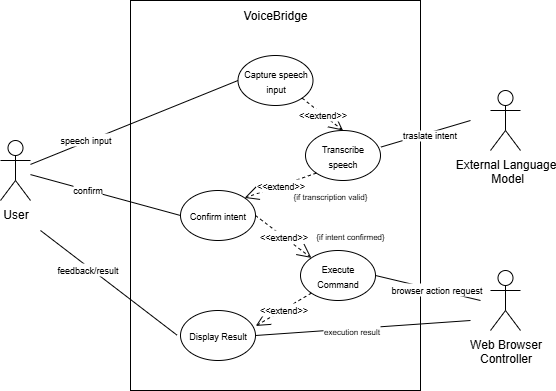
\includegraphics[width=1.1\textwidth]{..//imgs/VoiceBridge_use_case_diagram.png}
    \caption{VoiceBridge Use Case Diagram. Each ellipse represents a Product Use Case (PUC) corresponding to a major system function.}
    \label{fig:voicebridge-usecase}
\end{figure} 
\subsection{Product Use Case Table}
\begin{table}[H]
\centering
\caption{Product Use Case (PUC) Table}
\begin{tabularx}{\textwidth}{p{1.5cm}p{3cm}p{2.5cm}p{3cm}X}
\toprule
\textbf{PUC ID} & \textbf{Event Trigger} & \textbf{Input} & \textbf{Output} & \textbf{Description} \\
\midrule
PUC-1 & User speaks into microphone & Audio signal & Captured speech data & System listens for user speech input. \\
PUC-2 & Speech captured & Speech data & Text transcription & Converts impaired speech to text using trained model. \\
PUC-3 & Transcription complete & Transcribed text & Confirmation prompt / feedback & Seeks user confirmation to ensure correct interpretation. \\
PUC-4 & Intent confirmed & Confirmed command text & Browser command execution & Maps intent to actionable browser function. \\
PUC-5 & Command executed or error & System response & Success or error feedback to user & Provides feedback or prompts retry on failure. \\
\bottomrule
\end{tabularx}
\end{table}

\subsubsection{Individual Product Use Cases (PUC's)}
\section*{Product Use Cases}

This section defines the detailed Product Use Cases (PUCs) for the VoiceBridge system. Each PUC describes the interaction between the user and the system, including purpose, actors, triggers, inputs/outputs, and main scenarios.

\subsubsection*{PUC-1: Capture User Speech}
\textbf{Primary Actor:} User \\
\textbf{Trigger:} User begins speaking into the microphone. \\
\textbf{Precondition:} The microphone is connected and permissions are granted. \\
\textbf{Input:} Audio signal (live speech). \\
\textbf{Output:} Captured audio data stream. \\
\textbf{Postcondition:} Audio data is made available for processing by the ASR (Automatic Speech Recognition) module. \\

\textbf{Main Scenario:}
\begin{enumerate}
  \item User activates the VoiceBridge interface (e.g., presses a “Listen” button).
  \item The system listens through the microphone for input.
  \item The system captures the speech signal and stores it temporarily in memory.
  \item Captured data is sent to the speech-to-text module for processing.
\end{enumerate}

\textbf{Alternative Flow:}
\begin{itemize}
  \item If the microphone is unavailable or access is denied, the system displays an error prompt.
  \item User can retry after adjusting permissions or hardware connection.
\end{itemize}

\bigskip

\subsubsection*{PUC-2: Convert Speech to Text}
\textbf{Primary Actor:} System (Speech Recognition Module) \\
\textbf{Trigger:} Audio capture event completed. \\
\textbf{Input:} Captured speech data. \\
\textbf{Output:} Transcribed text. \\
\textbf{Postcondition:} Transcription results are ready for user confirmation. \\

\textbf{Main Scenario:}
\begin{enumerate}
  \item System processes the captured audio stream using a trained ASR model.
  \item Acoustic and linguistic features are extracted.
  \item Speech is converted to text and stored temporarily.
  \item Transcribed text is passed to the confirmation display.
\end{enumerate}

\textbf{Alternative Flow:}
\begin{itemize}
  \item If transcription confidence is below threshold, the system requests a repeat.
\end{itemize}

\bigskip

\subsubsection*{PUC-3: Confirm Transcription}
\textbf{Primary Actor:} User \\
\textbf{Trigger:} System displays transcribed text. \\
\textbf{Input:} Transcribed text. \\
\textbf{Output:} User confirmation or correction. \\

\textbf{Main Scenario:}
\begin{enumerate}
  \item The transcribed text is displayed to the user for verification.
  \item User confirms that the text is correct or requests reprocessing.
  \item System records the confirmation and proceeds to intent mapping.
\end{enumerate}

\textbf{Alternative Flow:}
\begin{itemize}
  \item If user rejects the transcription, the system returns to PUC-1 for re-input.
\end{itemize}

\bigskip

\subsubsection*{PUC-4: Map Intent to Browser Command}
\textbf{Primary Actor:} System (Command Mapping Module) \\
\textbf{Trigger:} User confirmation received. \\
\textbf{Input:} Confirmed command text. \\
\textbf{Output:} Actionable browser command. \\

\textbf{Main Scenario:}
\begin{enumerate}
  \item System parses confirmed text for intent (e.g., “open YouTube”).
  \item System searches for matching browser or OS command.
  \item Mapped command is passed to the execution layer.
\end{enumerate}

\textbf{Alternative Flow:}
\begin{itemize}
  \item If no matching command is found, the system provides suggestions.
\end{itemize}

\bigskip

\subsubsection*{PUC-5: Execute Command and Provide Feedback}
\textbf{Primary Actor:} System \\
\textbf{Trigger:} Actionable command received. \\
\textbf{Input:} Command representation (API or accessibility call). \\
\textbf{Output:} Visible browser or OS action, and feedback message. \\

\textbf{Main Scenario:}
\begin{enumerate}
  \item System executes the command using the browser’s API or accessibility layer.
  \item The target application or tab performs the intended action (e.g., opens a webpage).
  \item System provides visual and/or auditory feedback to confirm success.
\end{enumerate}

\textbf{Alternative Flow:}
\begin{itemize}
  \item If the command execution fails, an error message or retry option is displayed.
\end{itemize}


\section{Functional Requirements}
\subsection{Functional Requirements}

\subsection{FR1: Accept Speech Audio via Microphone}
\textbf{Description:} The system must capture live speech input from the user through a standard built-in or external microphone.\\
\textbf{Rationale:} Without microphone input, the system cannot acquire the user’s speech for transcription. Requiring only standard/built-in microphones keeps the solution accessible and affordable.\\
\textbf{Fit Criterion:} The system reliably detects and records audio from default OS microphone devices across Windows, macOS, iOS, and Android, with a minimum 16 kHz sampling rate.

\bigskip
\subsection{FR2: Convert Impaired Speech to Text with greater than or equal to 80\% Accuracy (MVP)}
\textbf{Description:} The system must process the captured audio and output a textual representation of the spoken utterance.\\
\textbf{Rationale:} Accurate transcription is the core functionality that enables communication and command execution. Without acceptable accuracy, the product fails its purpose.\\
\textbf{Fit Criterion:} In evaluation on a test dataset of impaired speech, transcription accuracy must reach at least 80\% word error rate (WER) reduction compared to baseline models, and achieve greater than or equal to 80\% accuracy for common commands.

\bigskip
\subsection{FR3: Display Transcription for Verification}
\textbf{Description:} The transcribed text must be displayed in real time on the user’s device interface.\\
\textbf{Rationale:} Transparent feedback allows the user to verify correctness, catch errors, and build trust in the system.\\
\textbf{Fit Criterion:} Every spoken input is displayed within 2 seconds as text on the UI, with at least 95\% consistency across trials.

\bigskip
\subsection{FR4: Map Text to Arbitrary Device Commands}
\textbf{Description:} The system must recognize when transcribed text corresponds to a predefined device action (e.g., “open amazon.ca,” “draft a new email”) and translate it into the appropriate command representation (API, CLI, or accessibility call).\\
\textbf{Rationale:} Mapping allows the system to extend beyond communication into real device control, empowering user independence.\\
\textbf{Fit Criterion:} For a test set of 50 predefined commands, the system maps user input to the correct command representation in at least 90\% of cases.

\bigskip
\subsection{FR5: Execute Commands on the Host Device}
\textbf{Description:} The system must execute the mapped commands through the host device’s accessibility framework or APIs, resulting in visible user action (e.g., app launch, scrolling, text entry).\\
\textbf{Rationale:} Without execution, the system remains a transcription tool only. Execution closes the loop between speech input and device interaction.\\
\textbf{Fit Criterion:} For each correctly recognized command, the intended system action occurs on the device within 2 seconds, with greater than or equal to 95\% reliability across test scenarios.


\section{Look and Feel Requirements}
\subsection{Appearance Requirements}
The interface shall have a clean and minimal design to reduce cognitive load. Key elements should be visually distinct, with consistent spacing, and color usage to support quick recognition of actions.

Since it’s a browser integration, the user interface should minimally interfere with the visibility of the content on the page. The interface should only capture the user’s attention as functionally needed (i.e., listening to user prompts, confirming user intent), but should otherwise blend in with the browser interface.

\subsection{Style Requirements}
The system shall maintain a professional and neutral visual style suitable for general workplace use. Colors, icons, and fonts should prioritize clarity over branding at this stage. Future iterations may incorporate custom styling or theming.


\section{Usability and Humanity Requirements}
\subsection{Ease of Use Requirements}
The system should minimize user effort by providing a simple, intuitive interface. Key actions should be accessible within 3-4 interactions, with clear feedback after each action.
\subsection{Personalization and Internationalization Requirements}
The system should support basic personalization (e.g., remembering user preferences) and allow easy adaptation for different languages or regions at a later stage. For the PoC, English support is sufficient.
\subsection{Learning Requirements}
The system should be learnable within 10 minutes without prior training or documentation. Users should be able to complete core tasks on their first attempt through the interfaces navigation tutorial upon first time launch. Additional documentation should be supplemental but not necessary. 
\subsection{Understandability and Politeness Requirements}
The system should use clear, direct, and neutral language in responses. Error messages or clarifications should remain polite and informative.
\subsection{Accessibility Requirements}
The interface should be navigable using standard assistive tools and offer clear text contrast and legible font sizes. Full accessibility compliance is not required at the PoC stage but should be feasible for future iterations.

\section{Performance Requirements}
\subsection{Speed and Latency Requirements}
Under normal operating conditions, latency requirements can be broken down into:

Speech interpretation: 5 s after end of utterance

Command generation \& execution: 10-15 seconds after end of speech interpretation
\subsection{Safety-Critical Requirements}
The system shall enforce guardrails to prevent unsafe or unintended actions, requiring validation and user confirmation for potentially disruptive operations, and provide warnings or fail-safes for errors.
\subsection{Precision or Accuracy Requirements}
ASR accuracy shall be at least 70\% in stationary noise conditions. The system shall achieve at least 80\% command recognition precision under stationary noise conditions for the PoC.
\subsection{Robustness or Fault-Tolerance Requirements}
The system shall remain stable under fluctuating network conditions and noisy input. Fallback mechanisms (e.g., retry logic, error messaging) shall ensure graceful issue handling.
\subsection{Capacity Requirements}
The system shall support at least 20 concurrent users without service degradation if the product is commercialized.
\subsection{Scalability or Extensibility Requirements}
The system architecture shall allow horizontal scaling to handle increased traffic and modular extensions fo new interaction capabilities. 
\subsection{Longevity Requirements}
The system shall be designed to operate reliably over a minimum of 5 years, with maintainable and updatable components to support long-term product evolution.

\section{Operational and Environmental Requirements}
\subsection{Expected Physical Environment}
The product shall be operable in a variety of typical office, home, or institutional environments where users perform their daily tasks. The system shall be robust to stationary background noise such as air conditioning, computer fans, and ambient hum. It is not required to reliably handle non-stationary noise, including multiple people speaking or sudden loud interruptions. No modifications to the host operating system, browser, or network configuration shall be required.
\subsection{Wider Environment Requirements}
The primary interface shall be web-based, accessible via standard web browsers, to maximize user accessibility and support flexible use cases.
\subsection{Requirements for Interfacing with Adjacent Systems}
\begin{enumerate}
    \item The system shall integrate with existing browser-based platforms and may interface with external language interpreter modules.
    \item Open-source components (e.g., browser interaction agents and libraries) may be incorporated, ensuring compatibility and maintainability.
\end{enumerate}

\subsection{Productization Requirements}
\begin{enumerate}
    \item The product shall be deployable for multiple users within an organization, supporting secure user accounts and personalized ASR profiles.
    \item The design shall allow packaging and distribution without requiring technical setup by end users. The product shall have straightforward installation or access via pre-configured web access and automatic model initialization.
    \item Productization shall include logging suitable for monitoring performance and usage in a hosted environment.
    \item The system shall include mechanisms for updates to features with minimal disruption to users.
\end{enumerate}
\subsection{Release Requirements}
The product shall follow a defined release cycle, providing minor updates quarterly and major updates semi-annually. Each release must maintain backward compatibility with user data, personalization settings, and existing features. Release planning will account for maintenance effort, compute resources, and compliance obligations.

\section{Maintainability and Support Requirements}
\subsection{Maintenance Requirements}
Code must be modular, documented, and testable to support scalability, debugging, and future updates. Maintenance must be possible by developers who were not the original authors. 
\subsection{Supportability Requirements}
The product shall provide an accessible Help Page and a Frequently Asked Questions (FAQ) section with clear instructions. It shall be displayed with high-contrast visuals, simple language, and auditory and visual aids. 
\subsection{Adaptability Requirements}
The system must run on common workplace platforms via a web browser, including Windows 10 or later, macOS 12 Monterey or later, and Linux distributions such as Ubuntu 20.04 LTS or later, supporting modern web browsers.

\section{Security Requirements}
\subsection{Access Requirements}
Only authorized end users shall be able to access personalized ASR features, voice command execution, and saved transcripts. Access shall be role-based:

\begin{itemize}
    \item \textbf{Primary users (end users):} can access their own data.
    \item \textbf{Secondary users (supervisors/SMEs):} may have read-only access to assist with support or troubleshooting.
    \item \textbf{Tertiary users (caregivers):} may have limited access to assist the end user, can view basic usage history and transcripts but cannot modify settings.
\end{itemize}

Access to external services (e.g., LLM APIs) shall be rate-limited to ensure system stability, control costs, and prevent abuse.
\subsection{Integrity Requirements}
The system must provide real-time confirmation and validation of commands before execution to ensure they match user intent. 
\subsection{Privacy Requirements}
The system must gather explicity user consent for storing voice and personal data. All user data used for model improvement must be anonymized. Database and personalized ASR models must maintain integrity through secure, versioned backups. Unauthorized changes or corruption of user data must be prevented. 
\subsection{Audit Requirements}
The system shall maintain secure logs of major actions and commands, including loging events, access to profile and personal data, and command execution failures. Logs shall be protected and retained in a secure database. 
\subsection{Immunity Requirements}
The system must be resilient to accidental misuse. It shall handle noisy input robustly, avoid executing unintended commands, and operate safely within rate limits to prevent resource overload. 

\section{Cultural Requirements}
\subsection{Cultural Requirements}
The system shall maintain a culturally neutral and respectful tone when prompting users, avoiding slang, bias, and discriminatory language. It must include ethical guardrails to prevent the generation of harmful content or execution of potentially dangerous commands.

It shall support inclusive and accessible design to serve users across diverse cultural backgrounds.

\section{Compliance Requirements}
\subsection{Legal Requirements}
The project shall comply with the Personal Information Protection and Electronic Documents Act (PIPEDA) regarding the collection, storage, and handling of personal information.

\subsection{Standards Compliance Requirements}
The application must comply with the Web Content Accessibility Guidelines (WCAG) 2.0, Level AA guidelines to ensure usability by individuals with disabilities.

\section{Requirements Likely and Unlikely to Change}

\subsection{Likely to Change}
\begin{itemize}
    \item \textbf{12.1 Speed \& Latency:} The system shall process speech input and return text in near real-time.\\
    \textit{Rationale:} Performance targets may improve as speech recognition and browser processing capabilities evolve.

    \item \textbf{14.3 Adaptability:} The system shall allow updates for new languages, user preferences, or accessibility features.\\
    \textit{Rationale:} Future user needs or new assistive technologies may require system modifications.

    \item \textbf{11.2 Personalization \& Internationalization:} The system shall support preferred voice, accent handling, and language selection.\\
    \textit{Rationale:} User preferences and supported languages are likely to expand over time.

    \item \textbf{12.6 Scalability \& Extensibility:} The system shall support an increasing number of concurrent users and new modules.\\
    \textit{Rationale:} User growth or additional features may require changes in infrastructure.

    \item \textbf{13.5 Release Requirements:} Updates shall be deployable on web browsers without downtime.\\
    \textit{Rationale:} Deployment strategies may change as development tools or environments evolve.

    \item \textbf{26.2 Personalized ASR Fine-Tuning:} The system shall allow individualized model tuning to improve transcription accuracy.\\
    \textit{Rationale:} Model improvements and user feedback may necessitate adjustments.


    \item \textbf{17.2 Standards Compliance Requirements:} System shall follow relevant industry standards.\\
    \textit{Rationale:} Standard adherence ensures safety, reliability, and credibility. As the product evolves, new features may require compliance with additional standards.
\end{itemize}

\subsection{Unlikely to Change}
\begin{itemize}
    \item \textbf{9.1 Functional Requirements:} The system shall accurately transcribe speech to text for users with speech impairments.\\
    \textit{Rationale:} Core transcription functionality is foundational and will not change.

    \item \textbf{10.1 Appearance:} Interface shall be clean, minimal, and visually organized to reduce cognitive load.\\
    \textit{Rationale:} Minimal and clear design is essential for accessibility and usability.

    \item \textbf{10.2 Style:} Interface shall use consistent fonts, spacing, and colors to support clarity.\\
    \textit{Rationale:} Visual consistency is fundamental for usability.

    \item \textbf{11.1 Ease of Use:} Users shall complete tasks with minimal steps or cognitive effort.\\
    \textit{Rationale:} Streamlined interaction is a core accessibility requirement.

    \item \textbf{15.3 Privacy Requirements:} User data shall be encrypted in the database and logs. \\
    \textit{Rationale:} Privacy protection is legally required and critical for trust, this requirement will not change.

    \item \textbf{17.1 Legal Requirements:} System shall comply with relevant regulations (e.g., PIPEDA).\\
    \textit{Rationale:} Compliance is mandatory for this project, must be complied with at all times.

\end{itemize}

\section{Open Issues}
The primary open issue is maintaining high ASR accuracy across the diverse and severe spectrum of dysarthric speech. This requires extensive training and validation data, as well as careful model tuning.


\section{Off-the-Shelf Solutions}
\subsection{Ready-Made Products}
The project will evaluate existing, specialized speech recognition models and applications (e.g., Whisper model and Project Euphonia) as performance baselines.

\subsection{Reusable Components}
Potential reused components could include existing Text-to-Speech (TTS) modules for feedback and LLMs to map user commands into structured actions.

\subsection{Products That Can Be Copied}
Open-source browser automation agents (e.g., The AI browser agent) may be integrated for command execution via voice input.


\section{New Problems}
\subsection{Effects on the Current Environment}
The product shall operate without modifying the user’s OS, browser, or network configuration. This separation prevents unintended impact from incorrect commands.

\subsection{Effects on the Installed Systems}
The product shall not bypass firewalls, alter security settings, access banned sites, install untrusted content, or perform any malware execution.

\subsection{Potential User Problems}
Due to the non-deterministic nature of dysarthric speech patterns, a user’s exact speech type may not be fully captured by the model, leading to higher training overhead for personalization before the system becomes reliably usable for them. Users may experience misinterpretations requiring retries, which can cause frustration.

\subsection{Limitations in the Anticipated Implementation Environment That May
Inhibit the New Product}
Variability in dysarthric speech may necessitate frequent retraining of ASR models.

Real-time performance varies between devices, depending on processing power and low-latency operation.
\subsection{Follow-Up Problems}
The local operation limits the ability to perform remote problem diagnosis if any issues arise.


\section{Tasks}
\subsection{Project Planning}
Breakdown of major tasks:

Our main tasks are centered on preparing the system by training and tuning the dysarthric ASR model, integrating the core command interpreter, designing the accessible interface, and conducting rigorous testing.
\subsection{Planning of the Development Phases}
A detailed schedule of development phases, milestones, and dependencies is outlined in the PoC and Development Plan.

\section{Migration to the New Product}
\subsection{Requirements for Migration to the New Product}
The system shall support new users with no prior ASR and interpreter experience through an onboarding process. 

The system shall support transitioning users migrating from an existing system by allowing for easy uploading of recordings of their speech training data.

\subsection{Data That Has to be Modified or Translated for the New System}
All previous transcripts, audio files, and personalization data shall be tied to secure user accounts.

Users shall be able to access their data from any supported device after logging in and authentication.

\section{Costs}
The primary costs for this product are related to machine learning computation and hosting. Development and training will initially leverage Compute Canada credits provided by the supervising research team, along with Colab Pro (CAD 13.99/month).

No external hosting costs are anticipated for the initial release; however, optional hosting may be required for commercial distribution and deployments. If hosting is included, approximate costs for cloud-based deployment on Google Cloud Platform (GCP) include: training and inference on GPUs (~\$50 CAD/month for pilot use), storage (~\$3 CAD/month), and minimal networking (~\$2–5 CAD/month). Costs scale with the number of users and training frequency. All estimates are approximate and intended for planning purposes.
\section{User Documentation and Training}
\subsection{User Documentation Requirements}
The system shall provide clear, accessible documentation, including an instructional guide and FAQ. (As noted in Section 14b, supporting requirements already cover this in detail.)

\subsection{Training Requirements}
Training shall not require formal instruction; the documentation and interface shall support self-directed onboarding.

\section{Waiting Room}
The system shall display launch, loading, or processing pages during transitions to provide users with clear feedback and reduce confusion during waiting periods.

\section{Ideas for Solution}

\subsection{Browser-Based Extensions}
The product is primarily web-based. Future considerations could include desktop or mobile apps to broaden the scope and accessibility (see Section 13 for environment and interface requirements).

\subsection{Personalized ASR Fine-Tuning}
Consider incremental model tuning paired with real-time streaming of speech input. This could be an approach to adapt to individual speech patterns while minimizing the training time overhead, related to the adaptability requirements discussed in earlier sections.

\subsection{LLM Command Mapping}
User intent parsing via context-aware LLMs could improve natural language command interpretation, as mentioned in Section 13.

\subsection{Noise Filtering}
Beyond stationary noise, adaptive filtering techniques could be adapted to enhance recognition in busier environments. Section 13 already specifies stationary noise handling.

\subsection{Open-Source Integrations}
Potential use of browser automation or voice control frameworks can be investigated, as mentioned in Section 16 for off-the-shelf solutions.

\subsection{Accessibility Enhancements}
Additional visual, auditory, or haptic cues for feedback and help features could enhance usability. Section 14 highlights basic supportability requirements that these enhancements would build on.

\subsection{Data Encryption}
Anonymized logging and privacy approaches can balance model improvement with privacy in mind. Section 15 discusses privacy requirements in detail.

\section{Requirements Phase-In Plan}

The following plan outlines the order in which the system requirements (9.1--17.2) will be addressed, aligned with project phases. Prioritization ensures that core functional requirements and critical non-functional requirements are validated first, with refinements and extensions added in later phases. Timelines for each phase are detailed in the Development Plan.

\subsection{Phase Definitions}

\begin{itemize}
    \item \textbf{Proof of Concept (PoC):} Validate feasibility of core functionality and critical performance metrics.
    \item \textbf{Revision 0:} Expand functionality, address usability, accessibility, and integrate initial security/privacy mechanisms.
    \item \textbf{Revision 1:} Final refinement, full productization, compliance, cultural, and maintainability requirements.
\end{itemize}

\subsection{Requirements Phase-In}

\begin{enumerate}
    % Functional Requirements
    \item \textbf{9.1 Functional Requirements:} Core system behaviors including input processing and basic transcription.\\
    \textit{Phase: PoC} \\
    \textit{Rationale:} Core functionality must be demonstrated to validate feasibility.

    % Look and Feel
    \item \textbf{10.1 Appearance Requirements:} Initial UI layout and interface elements.\\
    \textit{Phase: Revision 0} \\
    \textit{Rationale:} Visual interface can be refined after core functions are stable.

    \item \textbf{10.2 Style Requirements:} Consistent fonts, colors, and spacing.\\
    \textit{Phase: Revision 0} \\
    \textit{Rationale:} Enhances readability and user experience once functionality is proven.

    % Usability
    \item \textbf{11.1 Ease of Use Requirements:} Interface must be intuitive and straightforward.\\
    \textit{Phase: Revision 0} \\
    \textit{Rationale:} Important for usability testing, applied after functional PoC is complete.

    \item \textbf{11.2 Personalization and Internationalization Requirements:} Language/voice adaptations.\\
    \textit{Phase: Revision 1} \\
    \textit{Rationale:} Applied later when system is functionally stable.

    \item \textbf{11.3 Learning Requirements:} System should adapt to repeated user patterns.\\
    \textit{Phase: Revision 1} \\
    \textit{Rationale:} Machine learning or adaptation features require validated data pipelines.

    \item \textbf{11.4 Understandability and Politeness Requirements:} Feedback should be clear and respectful.\\
    \textit{Phase: Revision 0} \\
    \textit{Rationale:} Improves user experience during early testing.

    \item \textbf{11.5 Accessibility Requirements:} Interface supports assistive technologies.\\
    \textit{Phase: Revision 0} \\
    \textit{Rationale:} Early implementation ensures PoC testing is inclusive.

    % Performance
    \item \textbf{12.1 Speed and Latency Requirements:} System responds within acceptable time frames.\\
    \textit{Phase: PoC} \\
    \textit{Rationale:} Performance validation is crucial for feasibility.

    \item \textbf{12.2 Safety-Critical Requirements:} Ensure no harmful outputs or behaviors.\\
    \textit{Phase: PoC} \\
    \textit{Rationale:} Early validation prevents critical errors in PoC.

    \item \textbf{12.3 Precision or Accuracy Requirements:} Transcription must meet minimum WER/CER.\\
    \textit{Phase: PoC} \\
    \textit{Rationale:} Accuracy is the central PoC metric.

    \item \textbf{12.4 Robustness or Fault-Tolerance Requirements:} Handle errors gracefully.\\
    \textit{Phase: Revision 0} \\
    \textit{Rationale:} Necessary for reliable system use beyond PoC.

    \item \textbf{12.5 Capacity Requirements:} Support a small set of concurrent users/data.\\
    \textit{Phase: Revision 0} \\
    \textit{Rationale:} Ensure system can handle expected early usage.

    \item \textbf{12.6 Scalability or Extensibility Requirements:} System should allow future growth.\\
    \textit{Phase: Revision 1} \\
    \textit{Rationale:} Added after functional validation for longer-term planning.

    \item \textbf{12.7 Longevity Requirements:} Components maintainable over time.\\
    \textit{Phase: Revision 1} \\
    \textit{Rationale:} Stability and maintainability are late-stage concerns.

    % Operational & Environment
    \item \textbf{13.1 Expected Physical Environment:} System works on typical office/lab computers.\\
    \textit{Phase: PoC} \\
    \textit{Rationale:} Early testing on target devices is essential.

    \item \textbf{13.2 Wider Environment Requirements:} Browser compatibility.\\
    \textit{Phase: Revision 0} \\
    \textit{Rationale:} Once core functionality works, broaden environment testing.

    \item \textbf{13.3 Requirements for Interfacing with Adjacent Systems:} Integration points identified.\\
    \textit{Phase: Revision 1} \\
    \textit{Rationale:} External integration is late-phase after internal systems are stable.

    \item \textbf{13.4 Productization Requirements:} Ready for deployment.\\
    \textit{Phase: Revision 1} \\
    \textit{Rationale:} Combines all prior validations for release.

    \item \textbf{13.5 Release Requirements:} Packaging, distribution readiness.\\
    \textit{Phase: Revision 1} \\
    \textit{Rationale:} Ensures final delivery meets standards.

    % Maintainability & Support
    \item \textbf{14.1 Maintenance Requirements:} System maintainable.\\
    \textit{Phase: Revision 1} \\
    \textit{Rationale:} Implemented once core system is functional.

    \item \textbf{14.2 Supportability Requirements:} Technical support procedures.\\
    \textit{Phase: Revision 1} \\
    \textit{Rationale:} Late-stage requirement after main functionality.

    \item \textbf{14.3 Adaptability Requirements:} System can be upgraded.\\
    \textit{Phase: Revision 1} \\
    \textit{Rationale:} Flexibility comes after base system is validated.

    % Security
    \item \textbf{15.1 Access Requirements:} User roles and permissions.\\
    \textit{Phase: Revision 0} \\
    \textit{Rationale:} Early implementation secures initial PoC data.

    \item \textbf{15.2 Integrity Requirements:} Prevent tampering or corruption.\\
    \textit{Phase: Revision 0} \\
    \textit{Rationale:} Ensures reliable data handling.

    \item \textbf{15.3 Privacy Requirements:} Encrypt data in transit and at rest.\\
    \textit{Phase: Revision 0} \\
    \textit{Rationale:} Essential for user trust and legal compliance.

    \item \textbf{15.4 Audit Requirements:} Track critical system events.\\
    \textit{Phase: Revision 1} \\
    \textit{Rationale:} Auditing implemented after basic functionality and privacy are validated.

    \item \textbf{15.5 Immunity Requirements:} Protection from external attacks.\\
    \textit{Phase: Revision 1} \\
    \textit{Rationale:} Security hardening is a late-stage activity.

    % Cultural & Compliance
    \item \textbf{16.1 Cultural Requirements:} Respect cultural norms and sensitivities.\\
    \textit{Phase: Revision 1} \\
    \textit{Rationale:} Applied after all functional, UI, and content elements are stable.

    \item \textbf{17.1 Legal Requirements:} Comply with laws and regulations.\\
    \textit{Phase: Revision 1} \\
    \textit{Rationale:} Legal compliance verified after security, privacy, and functionality are validated.

    \item \textbf{17.2 Standards Compliance Requirements:} Follow industry standards.\\
    \textit{Phase: Revision 1} \\
    \textit{Rationale:} Ensures credibility and certification readiness at final stage.
\end{enumerate}


\newpage{}
\section*{Appendix --- Reflection}

The purpose of reflection questions is to give you a chance to assess your own
learning and that of your group as a whole, and to find ways to improve in the
future. Reflection is an important part of the learning process.  Reflection is
also an essential component of a successful software development process.  

Reflections are most interesting and useful when they're honest, even if the
stories they tell are imperfect. You will be marked based on your depth of
thought and analysis, and not based on the content of the reflections
themselves. Thus, for full marks we encourage you to answer openly and honestly
and to avoid simply writing ``what you think the evaluator wants to hear.''

Please answer the following questions.  Some questions can be answered on the
team level, but where appropriate, each team member should write their own
response:


\begin{enumerate}
  \item \textbf{What went well while writing this deliverable?} \\
  Organizing the SRS using the Volere template went surprisingly smoothly. Breaking down each requirement and writing clear rationales helped us think through the project in a structured way. Separating likely-to-change requirements from unlikely ones also made the document more readable and easier to navigate.

  \item \textbf{What pain points did you experience during this deliverable, and how did you resolve them?} \\
  Deciding which requirements might evolve over time versus those that would remain stable was a bit challenging. We resolved this by discussing potential future scenarios for the product and weighing Dr. Brodbeck’s expert guidance, which made our decisions much more confident.

  \item \textbf{How many of your requirements were inspired by speaking to your client(s) or their proxies?} \\
  Our requirements mostly came from our supervisor, Dr. Brodbeck, who is a linguistics expert and acts as our secondary stakeholder. We didn’t consult end-users directly, so the requirements reflect expert advice on accessibility, usability, and system functionality.

  \item \textbf{Which of the courses you have taken, or are currently taking, will help your team succeed with this project?} \\
  \begin{itemize}
    \item \textbf{SFWRENG 3RA3 – Software Requirements and Security:} Helped with writing clear Functional and Non-Functional Requirements and thinking about security, privacy, and reliability.
    \item \textbf{SFWRENG 4HC3 – Human-Computer Interfaces:} Provided a foundation for usability, stakeholder engagement, and accessibility considerations.
    \item Other courses in AI and Machine Learning are also valuable for speech recognition and natural language understanding.
  \end{itemize}

  \item \textbf{What knowledge and skills will the team need to successfully complete this project?} \\
  We need to improve on:
  \begin{itemize}
    \item Speech and linguistics for accessibility.
    \item Web development, particularly browser extensions.
    \item Machine learning for speech recognition.
    \item Accessibility standards and usability testing.
    \item Clear documentation and team coordination.
  \end{itemize}

  \item \textbf{How will each team member acquire these skills or knowledge?} \\
  \begin{itemize}
    \item \textbf{Speech and linguistics:} Weekly guidance from Dr. Brodbeck and reading related literature.
    \item \textbf{Web development/browser extensions:} Hands-on prototyping, online tutorials, and sharing coding tasks among team members.
    \item \textbf{Machine learning:} Experimenting with pre-trained speech models and following online courses.
    \item \textbf{Accessibility standards:} Reviewing WCAG guidelines and testing our prototype with assistive technologies.
  \end{itemize}
\end{enumerate}


\end{document}